	\paragraph{QuizziPedia::Front-End::Directives::ChangeLangDirective}
		
		\label{QuizziPedia::Front-End::Directives::ChangeLangDirective}
		
		\begin{figure}[ht]
			\centering
			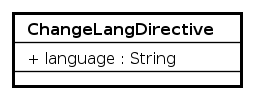
\includegraphics[scale=0.80,keepaspectratio]{UML/Classi/Front-End/QuizziPedia_Front-end_Directives_ChangeLangDirective.png}
			\caption{QuizziPedia::Front-End::Directives::ChangeLangDirective}
		\end{figure} \FloatBarrier
		
		\begin{itemize}
			\item \textbf{Descrizione}: \textit{directive\ped{G}} che mostra i bottoni che permettono di cambiare la lingua utilizzata all'interno dell'applicazione;
			\item \textbf{Utilizzo}: viene utilizzata per mostrare i bottoni che permettono all'utente di cambiare lingua all'interno dell'applicazione;
			\item \textbf{Relazioni con altre classi}: 
			\begin{itemize}
				\item \textbf{OUT \texttt{Index}}: \textit{view\ped{G}} generale dell'applicazione.
			\end{itemize}
			\item \textbf{Attributi}:
			\begin{itemize}
				\item \texttt{+ language: String} \\ Stringa che identifica la lingua in cui visualizzare i contenuti dell'applicazione. 
			\end{itemize}
		\end{itemize}